% Why Elastica Can Solve a PDE System with Explicit Arithmetic
% Standalone reference document — explains the method of lines, explicit vs implicit
% integration, and why Elastica's approach is valid for Cosserat rod dynamics

\documentclass[11pt]{article}

% ---------------------------------------------------------------------------
% Font and encoding
% ---------------------------------------------------------------------------
\usepackage{palatino}
\usepackage[T1]{fontenc}
\usepackage[utf8]{inputenc}

% ---------------------------------------------------------------------------
% Page layout
% ---------------------------------------------------------------------------
\usepackage[top=1in, bottom=1in, left=1.25in, right=1.25in]{geometry}
\usepackage{setspace}
\setstretch{1.15}
\setlength{\parindent}{1em}
\setlength{\parskip}{0.4em}

% ---------------------------------------------------------------------------
% Math
% ---------------------------------------------------------------------------
\usepackage{amsmath}
\usepackage{amssymb}
\usepackage{mathtools}
\usepackage{bm}

% ---------------------------------------------------------------------------
% Figures and tables
% ---------------------------------------------------------------------------
\usepackage{booktabs}
\usepackage{float}
\usepackage{array}

% ---------------------------------------------------------------------------
% Colors, boxes, and hyperlinks
% ---------------------------------------------------------------------------
\usepackage{xcolor}
\usepackage[most]{tcolorbox}
\usepackage[hidelinks]{hyperref}

% ---------------------------------------------------------------------------
% Lists
% ---------------------------------------------------------------------------
\usepackage{enumitem}
\setlist[itemize]{nosep, topsep=0.3em, itemsep=0.2em}

% ---------------------------------------------------------------------------
% Section formatting
% ---------------------------------------------------------------------------
\usepackage{titlesec}
\titlespacing*{\section}{0pt}{1.2em}{0.6em}
\titlespacing*{\subsection}{0pt}{0.9em}{0.3em}
\titlespacing*{\subsubsection}{0pt}{0.7em}{0.2em}

% ---------------------------------------------------------------------------
% TikZ for diagrams
% ---------------------------------------------------------------------------
\usepackage{tikz}
\usetikzlibrary{arrows.meta, positioning, calc, decorations.pathreplacing}

% ---------------------------------------------------------------------------
% Custom commands
% ---------------------------------------------------------------------------
\newcommand{\vect}[1]{\mathbf{#1}}
\newcommand{\mat}[1]{\mathbf{#1}}
\newcommand{\Real}{\mathbb{R}}
\newcommand{\ddt}[1]{\frac{\partial #1}{\partial t}}
\newcommand{\dds}[1]{\frac{\partial #1}{\partial s}}
\newcommand{\dd}[2]{\frac{d #1}{d #2}}

% ---------------------------------------------------------------------------
\begin{document}
% ---------------------------------------------------------------------------

\begin{center}
  {\Large\bfseries Why Elastica Solves PDEs with Explicit Arithmetic} \\[0.5em]
  {\large The Method of Lines, Explicit Integration, \\
  and Sequential Evaluation as a PDE Solution Strategy} \\[1.5em]
  \textit{Snake-HRL Project --- Reference Document}
\end{center}

\vspace{1em}

% ===================================================================
\section{The Question}
\label{sec:question}
% ===================================================================

The Cosserat rod model is governed by partial differential equations (PDEs) in two independent variables --- arc length $s$ and time $t$.
Yet PyElastica's simulation loop contains no iterative solver, no matrix inversion, and no convergence check.
Each substep is a sequence of explicit arithmetic operations: compute tangent vectors, evaluate constitutive laws, assemble forces, update velocities, advance positions.
Three natural questions arise:

\begin{enumerate}
  \item Why is Elastica's method called ``explicit''?
  \item What is the standard way to solve a PDE system, and which approach qualifies as a ``solver'' in the traditional sense?
  \item How can Elastica solve a PDE system through sequential evaluation --- that is, without ever solving an equation?
\end{enumerate}

% ===================================================================
\section{Standard Approaches to Solving PDE Systems}
\label{sec:approaches}
% ===================================================================

A PDE initial--boundary value problem (IBVP) is a continuous mathematical object.
No computer can represent continuous functions directly, so \emph{every} numerical method must discretize the problem.
The three dominant discretization families are:

\begin{enumerate}
  \item \textbf{Finite differences (FD):} Replace derivatives with algebraic differences on a grid.
  \item \textbf{Finite elements (FEM):} Approximate the solution as a linear combination of basis functions and enforce the PDE in a weak (integral) sense.
  \item \textbf{Spectral methods:} Expand the solution in global basis functions (Fourier, Chebyshev) and enforce the PDE in frequency space.
\end{enumerate}

All three families share a common structure: they convert the continuous PDE into a discrete system (algebraic equations or ODEs) that a computer can evaluate.

\subsection{Time-dependent PDEs: space first or time first?}

For a PDE with both spatial and temporal derivatives, there are two discretization strategies:

\begin{table}[H]
\centering
\renewcommand{\arraystretch}{1.3}
\begin{tabular}{@{}lp{5.2cm}p{5.2cm}@{}}
\toprule
\textbf{Strategy} & \textbf{Procedure} & \textbf{Result} \\
\midrule
\textbf{Method of lines} \newline (semi-discrete) &
  Discretize space first. \newline Leave time continuous. &
  System of ODEs in time: $\dot{\vect{s}} = \vect{g}(\vect{s}, t)$ \\[6pt]
\textbf{Full discretization} \newline (Rothe's method) &
  Discretize time first. \newline Solve spatial BVP at each timestep. &
  Sequence of elliptic problems: $\mathcal{L}_h\,\vect{u}^{n+1} = \vect{b}^n$ \\
\bottomrule
\end{tabular}
\end{table}

\noindent
PyElastica uses the \textbf{method of lines}: spatial derivatives are replaced by finite differences on a staggered grid, producing an ODE system that is then integrated in time.

\subsection{Which approach is the ``typical solver''?}

In computational solid mechanics (the field that Cosserat rod simulation belongs to), the dominant paradigm is implicit FEM:

\begin{itemize}
  \item Discretize space with finite elements.
  \item Discretize time with an implicit scheme (backward Euler, Newmark, generalized-$\alpha$).
  \item At each timestep, solve a nonlinear algebraic system via Newton's method, which requires assembling and factorizing a tangent stiffness matrix.
\end{itemize}

This is what DisMech does, and it is the approach most engineers mean when they say ``PDE solver.''
The Newton iteration is the core computational engine: it solves an equation (the nonlinear residual $\vect{g}(\vect{q}_{n+1}) = \vect{0}$) at every timestep.

PyElastica departs from this paradigm by using an \emph{explicit} time integrator, which avoids the Newton solve entirely.

% ===================================================================
\section{What Discretization Means and How It Works}
\label{sec:discretization}
% ===================================================================

A PDE describes how a continuous field $\vect{u}(s, t)$ evolves over a continuous domain.
A computer cannot store or manipulate continuous functions --- it works with finite arrays of numbers.
\textbf{Discretization} is the process of replacing the infinite-dimensional continuous problem with a finite-dimensional discrete problem that a computer can evaluate.

There are two things to discretize: (i)~the \emph{domain} (where the solution lives), and (ii)~the \emph{operators} (the derivatives that act on the solution).
Once both are discretized, the PDE becomes a system of algebraic equations or ODEs in a finite number of unknowns.

\subsection{Discretizing the domain: from fields to arrays}

The continuous Cosserat rod is parameterized by arc length $s \in [0, L]$.
At every point $s$, the rod carries a position vector $\vect{x}(s) \in \Real^3$, a velocity $\vect{v}(s) \in \Real^3$, a director frame $\mat{Q}(s) \in \Real^{3 \times 3}$, and an angular velocity $\bm{\omega}(s) \in \Real^3$.
This is an infinite-dimensional object: there are uncountably many points $s$, each carrying multiple vector fields.

Spatial discretization replaces this continuum with a \emph{finite set of sample points} (a mesh or grid).
For Cosserat rods, the natural choice is a staggered grid:

\begin{center}
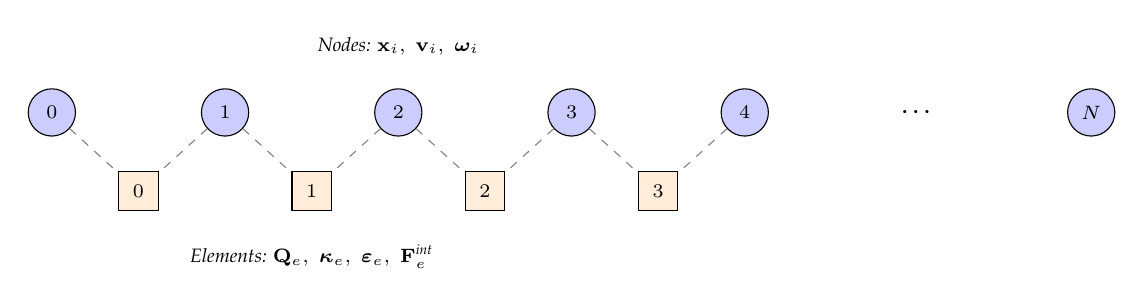
\begin{tikzpicture}[
  node/.style={circle, draw, fill=blue!20, minimum size=6mm, inner sep=0pt, font=\scriptsize},
  elem/.style={rectangle, draw, fill=orange!15, minimum size=5mm, inner sep=0pt, font=\scriptsize},
  lbl/.style={font=\scriptsize\itshape}
]
  % Nodes
  \foreach \i in {0,...,4} {
    \node[node] (n\i) at (2.2*\i, 0) {$\i$};
  }
  \node at (2.2*5, 0) {\dots};
  \node[node] (nN) at (2.2*6, 0) {$N$};

  % Elements (between nodes)
  \foreach \i [evaluate=\i as \j using int(\i+1)] in {0,...,3} {
    \node[elem] (e\i) at ($(n\i)!0.5!(n\j) + (0, -1.0)$) {$\i$};
    \draw[dashed, gray] (n\i) -- (e\i);
    \draw[dashed, gray] (n\j) -- (e\i);
  }

  % Labels
  \node[lbl, above=3mm of n2] {Nodes: $\vect{x}_i,\; \vect{v}_i,\; \bm{\omega}_i$};
  \node[lbl, below=3mm of e1] {Elements: $\mat{Q}_e,\; \bm{\kappa}_e,\; \bm{\varepsilon}_e,\; \vect{F}_e^{\text{int}}$};
\end{tikzpicture}
\end{center}

\begin{itemize}
  \item \textbf{Nodes} ($i = 0, \dots, N$): carry position $\vect{x}_i$, translational velocity $\vect{v}_i$, and angular velocity $\bm{\omega}_i$.
    These are the \emph{kinematic} quantities --- they describe where the rod is and how it moves.
  \item \textbf{Elements} ($e = 0, \dots, N_e - 1$, connecting adjacent nodes): carry the director frame $\mat{Q}_e$, strains $\bm{\varepsilon}_e$, curvatures $\bm{\kappa}_e$, and internal forces $\vect{F}_e^{\text{int}}$.
    These are the \emph{constitutive} quantities --- they describe how the rod deforms and what forces arise from that deformation.
\end{itemize}

After this step, the continuous field $\vect{u}(s, t)$ is replaced by a finite state vector:
\begin{equation}
  \vect{s}(t) = \bigl(\vect{x}_0,\, \dots,\, \vect{x}_N,\;
                       \vect{v}_0,\, \dots,\, \vect{v}_N,\;
                       \bm{\omega}_0,\, \dots,\, \bm{\omega}_N,\;
                       \mat{Q}_0,\, \dots,\, \mat{Q}_{N_e-1}\bigr)
  \;\in\; \Real^{d}
  \label{eq:state-vector}
\end{equation}
The infinite-dimensional function space has been replaced by $\Real^d$ (here $d = 124$ for the default 21-node rod).

\subsection{Discretizing the operators: from derivatives to differences}

The PDE contains spatial derivatives like $\partial \vect{F} / \partial s$.
These operate on the continuous field --- they measure how a quantity changes over an infinitesimally small interval $ds$.
On a discrete grid, there is no infinitesimal interval; the smallest distance is the element length $\Delta s = \ell_e$.

A \textbf{finite difference} approximates the derivative by a ratio of differences between neighboring grid values:
\begin{equation}
  \dds{\vect{F}}\bigg|_{s_i}
  \;\approx\;
  \frac{\vect{F}_{e_i} - \vect{F}_{e_{i-1}}}{\Delta s}
  \;=\;
  \bigl[\mat{D}^T \vect{F}_e\bigr]_i
  \label{eq:fd-approximation}
\end{equation}

This is the simplest case (central difference on the staggered grid), but the principle is general: \emph{every spatial derivative becomes a weighted sum of neighboring values}.
In matrix notation, the derivative operator $\partial/\partial s$ becomes a sparse matrix $\mat{D}$ or $\mat{D}^T$, and applying the derivative becomes a matrix--vector product.

The key difference operators for the Cosserat rod are:

\begin{table}[H]
\centering
\renewcommand{\arraystretch}{1.4}
\begin{tabular}{@{}p{3.8cm}p{3.5cm}p{4.5cm}@{}}
\toprule
\textbf{Continuous operator} & \textbf{Discrete operator} & \textbf{Structure} \\
\midrule
$\partial/\partial s$ (node $\to$ element) &
  $\mat{D}$ &
  Bidiagonal: $D_{e,i} = \delta_{e,i+1} - \delta_{e,i}$ \\
$\partial/\partial s$ (element $\to$ node) &
  $\mat{D}^T$ &
  Transpose of $\mat{D}$ \\
Average (node $\to$ Voronoi) &
  $\mat{A}_v$ &
  Tridiagonal: weighted mean of neighbors \\
Difference (node $\to$ Voronoi) &
  $\mat{D}_v$ &
  Bidiagonal on Voronoi cells \\
\bottomrule
\end{tabular}
\end{table}

\noindent
These matrices are extremely sparse --- each row has at most two or three nonzero entries.
A matrix--vector product $\mat{D}^T \vect{F}_e$ involves only $O(N)$ additions and multiplications, not a system of equations.

\subsection{Worked example: from PDE to arithmetic on five nodes}

To make the discretization concrete, consider a short rod segment with five nodes ($N = 4$, $N_e = 4$) and uniform element length $\Delta s$.
We trace how the continuous linear momentum PDE becomes a sequence of arithmetic operations.

\paragraph{Step 0: The continuous PDE.}
The linear momentum balance for the Cosserat rod is:
\begin{equation}
  \rho A \ddt{\vect{v}} = \dds{\vect{F}} + \vect{f}_{\text{ext}}
  \label{eq:pde-momentum}
\end{equation}
This says: the acceleration at every point $s$ equals the spatial gradient of internal force plus external force.
Both sides are continuous functions of $s$ and $t$.

\begin{tcolorbox}[colback=blue!3, colframe=blue!30, title={\small Step 0 --- What we have}, fonttitle=\bfseries\small]
\begin{minipage}[t]{0.55\linewidth}
\textbf{Domain:} The rod is a continuous curve parameterized by arc length $s \in [0, L]$.\\[2pt]
\textbf{Unknowns:} $\vect{v}(s, t)$ and $\vect{F}(s, t)$ are \emph{fields} --- they assign a vector to every point $s$ on the rod, at every instant $t$.
There are \emph{uncountably many} values.\\[2pt]
\textbf{Derivatives:} $\partial \vect{F}/\partial s$ is a true derivative --- a limit of $(\vect{F}(s+h) - \vect{F}(s))/h$ as $h \to 0$.
\end{minipage}\hfill
\begin{minipage}[t]{0.4\linewidth}
\centering
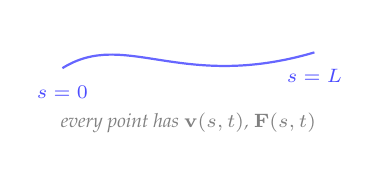
\begin{tikzpicture}[>=Stealth]
  \draw[thick, blue!60] (0,0) .. controls (0.8, 0.5) and (1.5, -0.3) .. (3.2, 0.2);
  \node[font=\scriptsize, blue!70] at (0, -0.3) {$s=0$};
  \node[font=\scriptsize, blue!70] at (3.2, -0.1) {$s=L$};
  \node[font=\scriptsize\itshape, black!50] at (1.6, -0.7) {every point has $\vect{v}(s,t)$, $\vect{F}(s,t)$};
\end{tikzpicture}
\end{minipage}
\end{tcolorbox}

\paragraph{Step 1: Discretize the domain.}
Replace the continuous rod with five nodes at positions $s_0, s_1, s_2, s_3, s_4$ and four elements connecting them:

\begin{center}
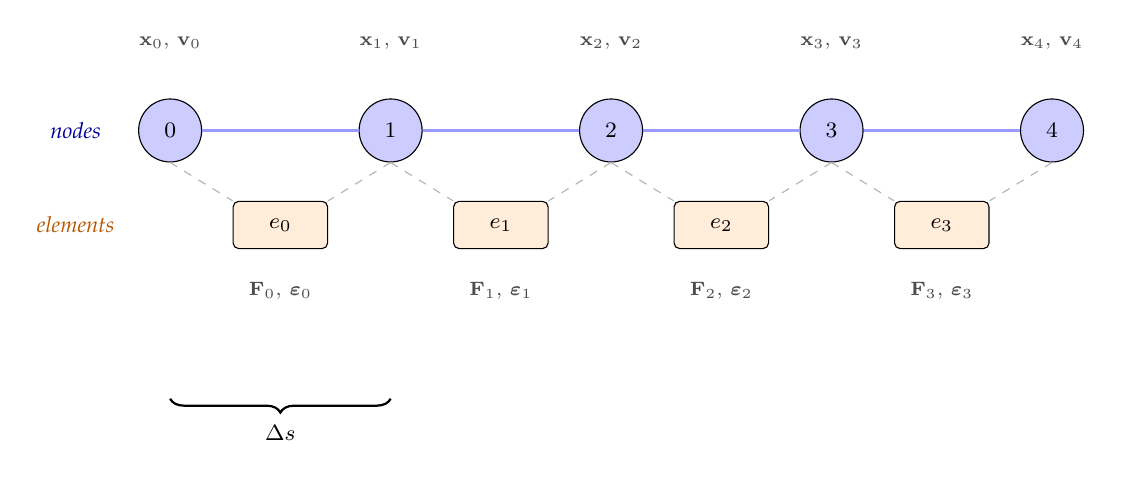
\begin{tikzpicture}[
  nd/.style={circle, draw, fill=blue!20, minimum size=8mm, inner sep=0pt, font=\footnotesize},
  el/.style={rectangle, draw, fill=orange!15, rounded corners=2pt, minimum width=12mm, minimum height=6mm, inner sep=0pt, font=\footnotesize},
  qty/.style={font=\scriptsize, text=black!70},
  brace/.style={decorate, decoration={brace, amplitude=5pt, mirror}},
  >=Stealth
]
  % Nodes
  \foreach \i in {0,...,4} {
    \node[nd] (n\i) at (2.8*\i, 0) {$\i$};
  }

  % Node quantities (above)
  \foreach \i in {0,...,4} {
    \node[qty, above=5mm of n\i] {$\vect{x}_\i,\, \vect{v}_\i$};
  }

  % Elements (below, between nodes)
  \foreach \i [evaluate=\i as \j using int(\i+1)] in {0,...,3} {
    \node[el] (e\i) at ($(n\i)!0.5!(n\j) + (0, -1.2)$) {$e_\i$};
    \draw[dashed, gray!60] (n\i.south) -- (e\i.north west);
    \draw[dashed, gray!60] (n\j.south) -- (e\i.north east);
  }

  % Element quantities (below elements)
  \foreach \i in {0,...,3} {
    \node[qty, below=3mm of e\i] {$\vect{F}_\i,\, \bm{\varepsilon}_\i$};
  }

  % Rod segments connecting nodes
  \foreach \i [evaluate=\i as \j using int(\i+1)] in {0,...,3} {
    \draw[thick, blue!40] (n\i) -- (n\j);
  }

  % Delta s brace
  \draw[brace, thick] ($(n0.south) + (0, -3.0)$) -- node[below=6pt, font=\footnotesize] {$\Delta s$} ($(n1.south) + (0, -3.0)$);

  % Labels
  \node[font=\footnotesize\itshape, blue!60!black] at (-1.2, 0) {nodes};
  \node[font=\footnotesize\itshape, orange!70!black] at (-1.2, -1.2) {elements};
\end{tikzpicture}
\end{center}

\noindent
The continuous velocity field $\vect{v}(s, t)$ becomes five velocity vectors:
\[
  \vect{v}(s, t) \;\longrightarrow\; \vect{v}_0(t),\; \vect{v}_1(t),\; \vect{v}_2(t),\; \vect{v}_3(t),\; \vect{v}_4(t)
\]
Similarly, the internal force field becomes four element force vectors $\vect{F}_0, \vect{F}_1, \vect{F}_2, \vect{F}_3$ (one per element).

\begin{tcolorbox}[colback=white, colframe=black!40, title={\small Step 1 --- Continuous vs.\ discretized domain}, fonttitle=\bfseries\small]
\begin{minipage}[t]{0.47\linewidth}
\centering\textbf{Continuous (before)}\\[4pt]
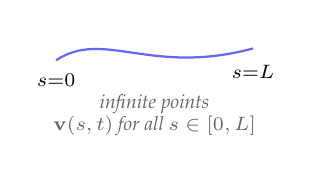
\begin{tikzpicture}[>=Stealth]
  \draw[thick, blue!60] (0,0) .. controls (0.6, 0.4) and (1.2, -0.2) .. (2.5, 0.15);
  \node[font=\scriptsize] at (0, -0.25) {$s{=}0$};
  \node[font=\scriptsize] at (2.5, -0.15) {$s{=}L$};
  \node[font=\scriptsize\itshape, text=black!60, align=center] at (1.25, -0.7)
    {infinite points\\$\vect{v}(s,t)$ for all $s \in [0,L]$};
\end{tikzpicture}
\end{minipage}\hfill
\vrule width 0.4pt\hfill
\begin{minipage}[t]{0.47\linewidth}
\centering\textbf{Discretized (after)}\\[4pt]
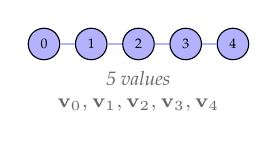
\begin{tikzpicture}[>=Stealth,
  nd/.style={circle, fill=blue!30, draw, inner sep=0pt, minimum size=4mm, font=\tiny}]
  \foreach \i in {0,...,4} {
    \node[nd] (n\i) at (0.6*\i, 0) {\i};
  }
  \foreach \i [evaluate=\i as \j using int(\i+1)] in {0,...,3} {
    \draw[thick, blue!30] (n\i) -- (n\j);
  }
  \node[font=\scriptsize\itshape, text=black!60, align=center] at (1.2, -0.6)
    {5 values\\$\vect{v}_0, \vect{v}_1, \vect{v}_2, \vect{v}_3, \vect{v}_4$};
\end{tikzpicture}
\end{minipage}

\smallskip
\noindent\textit{What changed:} The continuous field $\vect{v}(s,t)$ defined at uncountably many points was replaced by a finite list of 5 vectors.
The rod's state went from an infinite-dimensional function to a finite-dimensional vector $\vect{s} \in \Real^{124}$.
No information is lost about these 5 points; the approximation is that we \emph{ignore} what happens between them.
\end{tcolorbox}

\paragraph{Step 2: Discretize the spatial derivative.}
The continuous derivative $\partial \vect{F} / \partial s$ is replaced by finite differences.
For an interior node $i$, the force gradient is approximated by the difference of the forces in the two adjacent elements:
\begin{equation}
  \dds{\vect{F}}\bigg|_{s_i} \;\approx\; \frac{\vect{F}_{e_i} - \vect{F}_{e_{i-1}}}{\Delta s}
  \label{eq:fd-force}
\end{equation}
Writing this out for every node (with boundary treatment at the endpoints):
\begin{equation}
  \underbrace{\begin{pmatrix}
    [\partial_s \vect{F}]_0 \\ [\partial_s \vect{F}]_1 \\ [\partial_s \vect{F}]_2 \\ [\partial_s \vect{F}]_3 \\ [\partial_s \vect{F}]_4
  \end{pmatrix}}_{\text{nodal force gradients}}
  = \frac{1}{\Delta s}
  \underbrace{\begin{pmatrix}
    -1 &  0 &  0 &  0 \\
     1 & -1 &  0 &  0 \\
     0 &  1 & -1 &  0 \\
     0 &  0 &  1 & -1 \\
     0 &  0 &  0 &  1
  \end{pmatrix}}_{\mat{D}^T \;\text{(5$\times$4)}}
  \underbrace{\begin{pmatrix}
    \vect{F}_0 \\ \vect{F}_1 \\ \vect{F}_2 \\ \vect{F}_3
  \end{pmatrix}}_{\text{element forces}}
  \label{eq:DT-example}
\end{equation}

\noindent
The following diagram shows what this matrix--vector product does for node~2:

\begin{center}
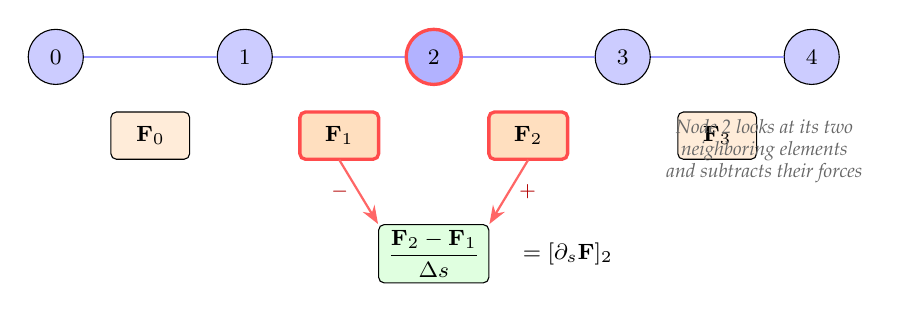
\begin{tikzpicture}[
  nd/.style={circle, draw, fill=blue!20, minimum size=7mm, inner sep=0pt, font=\footnotesize},
  el/.style={rectangle, draw, fill=orange!15, rounded corners=2pt, minimum width=10mm, minimum height=6mm, inner sep=0pt, font=\footnotesize},
  result/.style={rectangle, draw, fill=green!12, rounded corners=2pt, minimum width=14mm, minimum height=7mm, inner sep=2pt, font=\footnotesize},
  op/.style={font=\scriptsize, text=red!70!black},
  >=Stealth
]
  % Nodes
  \foreach \i in {0,...,4} {
    \node[nd] (n\i) at (2.4*\i, 0) {$\i$};
  }
  \foreach \i [evaluate=\i as \j using int(\i+1)] in {0,...,3} {
    \draw[thick, blue!40] (n\i) -- (n\j);
  }

  % Elements with forces
  \foreach \i [evaluate=\i as \j using int(\i+1)] in {0,...,3} {
    \node[el] (e\i) at ($(n\i)!0.5!(n\j) + (0, -1.0)$) {$\vect{F}_\i$};
  }

  % Highlight the two elements that node 2 uses
  \node[el, draw=red!70, line width=1.2pt, fill=orange!25] at (e1) {$\vect{F}_1$};
  \node[el, draw=red!70, line width=1.2pt, fill=orange!25] at (e2) {$\vect{F}_2$};

  % Highlight node 2
  \node[nd, draw=red!70, line width=1.2pt, fill=blue!30] at (n2) {$2$};

  % Arrows from elements to result
  \node[result] (res) at (4.8, -2.5) {$\displaystyle\frac{\vect{F}_2 - \vect{F}_1}{\Delta s}$};

  \draw[->, thick, red!60] (e1.south) -- node[left, op] {$-$} (res.north west);
  \draw[->, thick, red!60] (e2.south) -- node[right, op] {$+$} (res.north east);

  % Label
  \node[font=\footnotesize, right=3mm of res] {$= [\partial_s \vect{F}]_2$};

  % Annotation
  \node[font=\scriptsize\itshape, text=black!60, align=center] at (9.0, -1.2)
    {Node 2 looks at its two\\neighboring elements\\and subtracts their forces};
\end{tikzpicture}
\end{center}

\noindent
The continuous derivative $\partial \vect{F}/\partial s$ became a \emph{matrix--vector multiply}.
For node~2, the result is simply $(\vect{F}_2 - \vect{F}_1)/\Delta s$ --- the difference of two neighboring values, divided by the spacing.
This is \textbf{arithmetic}, not an equation to solve.

\begin{tcolorbox}[colback=white, colframe=black!40, title={\small Step 2 --- Continuous vs.\ discretized spatial derivative}, fonttitle=\bfseries\small]
\begin{minipage}[t]{0.47\linewidth}
\centering\textbf{Continuous (before)}
\[
  \dds{\vect{F}}\bigg|_{s_2} = \lim_{h \to 0} \frac{\vect{F}(s_2 + h) - \vect{F}(s_2)}{h}
\]
Requires knowing $\vect{F}$ at \emph{infinitesimally close} points.
This is a limit --- cannot be computed on a discrete grid.
\end{minipage}\hfill
\vrule width 0.4pt\hfill
\begin{minipage}[t]{0.47\linewidth}
\centering\textbf{Discretized (after)}
\[
  \dds{\vect{F}}\bigg|_{s_2} \approx \frac{\vect{F}_2 - \vect{F}_1}{\Delta s}
\]
Uses only two neighboring force values that we already have.
This is a subtraction followed by a division.
\end{minipage}

\smallskip
\noindent\textit{What changed:} The infinitesimal limit $h \to 0$ was replaced by a \emph{finite} difference with step size $\Delta s$.
The approximation improves as $\Delta s$ shrinks (more nodes), with error proportional to $(\Delta s)^2$ for a centered scheme.
The key point: the derivative, which is defined as a limit and cannot be computed exactly on a computer, became a subtraction of two known numbers.
\end{tcolorbox}

\paragraph{Step 3: Compute element forces from the constitutive law.}
The element forces $\vect{F}_e$ are not free variables --- they are determined by the current deformation.
The constitutive law relates force to strain:
\begin{equation}
  \vect{F}_e = \mat{S}\,(\bm{\varepsilon}_e - \bm{\varepsilon}_e^{\text{rest}})
  \label{eq:constitutive-example}
\end{equation}
where $\mat{S} = \mathrm{diag}(GA,\, GA,\, EA)$ is the stiffness matrix (shear, shear, stretch), and the strain is computed from node positions:
\begin{equation}
  \bm{\varepsilon}_e = \mat{Q}_e^T \frac{\vect{x}_{e+1} - \vect{x}_e}{\ell_e^{\text{rest}}}
  \label{eq:strain-example}
\end{equation}
Again, this is pure arithmetic: subtract two position vectors, divide by rest length, rotate into the local frame, multiply by stiffness.
The following diagram traces the computation for element~1:

\begin{center}
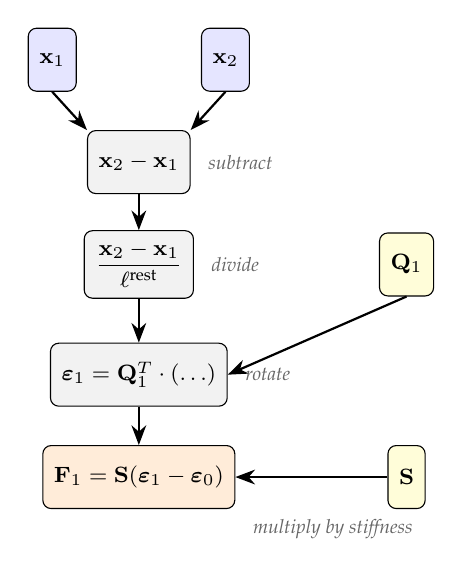
\begin{tikzpicture}[
  box/.style={rectangle, draw, rounded corners=3pt, minimum height=8mm, inner sep=4pt, font=\footnotesize, align=center},
  arr/.style={-{Stealth[length=2.5mm]}, thick},
  op/.style={font=\scriptsize\itshape, text=black!60},
  >=Stealth
]
  % Input: two node positions
  \node[box, fill=blue!10] (x1) at (0, 0) {$\vect{x}_1$};
  \node[box, fill=blue!10] (x2) at (2.2, 0) {$\vect{x}_2$};

  % Subtract
  \node[box, fill=gray!10] (diff) at (1.1, -1.3) {$\vect{x}_2 - \vect{x}_1$};
  \draw[arr] (x1.south) -- (diff.north west);
  \draw[arr] (x2.south) -- (diff.north east);
  \node[op, right=1mm of diff] {subtract};

  % Divide by rest length
  \node[box, fill=gray!10] (tang) at (1.1, -2.6) {$\displaystyle\frac{\vect{x}_2 - \vect{x}_1}{\ell^{\text{rest}}}$};
  \draw[arr] (diff) -- (tang);
  \node[op, right=1mm of tang] {divide};

  % Rotate into local frame
  \node[box, fill=yellow!15] (Q) at (4.5, -2.6) {$\mat{Q}_1$};
  \node[box, fill=gray!10] (strain) at (1.1, -4.0) {$\bm{\varepsilon}_1 = \mat{Q}_1^T \cdot (\ldots)$};
  \draw[arr] (tang) -- (strain);
  \draw[arr] (Q.south) -- (strain.east);
  \node[op, right=1mm of strain] {rotate};

  % Constitutive law
  \node[box, fill=yellow!15] (S) at (4.5, -5.3) {$\mat{S}$};
  \node[box, fill=orange!15] (F) at (1.1, -5.3) {$\vect{F}_1 = \mat{S}(\bm{\varepsilon}_1 - \bm{\varepsilon}_0)$};
  \draw[arr] (strain) -- (F);
  \draw[arr] (S) -- (F);
  \node[op, right=1mm of F.south east, anchor=north west] {multiply by stiffness};
\end{tikzpicture}
\end{center}

\noindent
Every box is computed from the boxes above it using basic operations (subtract, divide, rotate, multiply).
The yellow boxes ($\mat{Q}_1$, $\mat{S}$) are known quantities from the current state and material properties.

\begin{tcolorbox}[colback=white, colframe=black!40, title={\small Step 3 --- Continuous vs.\ discretized constitutive law}, fonttitle=\bfseries\small]
\begin{minipage}[t]{0.47\linewidth}
\centering\textbf{Continuous (before)}
\[
  \vect{F}(s, t) = \mat{S}\!\left[\mat{Q}(s,t)^T \dds{\vect{x}}(s,t) - \bm{\varepsilon}_0\right]
\]
The strain $\partial \vect{x}/\partial s$ is again a spatial derivative --- a limit.
$\mat{Q}(s,t)$ is a rotation field defined at every point.
This requires the continuous tangent vector everywhere.
\end{minipage}\hfill
\vrule width 0.4pt\hfill
\begin{minipage}[t]{0.47\linewidth}
\centering\textbf{Discretized (after)}
\[
  \vect{F}_1 = \mat{S}\!\left[\mat{Q}_1^T \frac{\vect{x}_2 - \vect{x}_1}{\ell^{\text{rest}}} - \bm{\varepsilon}_0\right]
\]
The spatial derivative $\partial \vect{x}/\partial s$ was replaced by $(\vect{x}_2 - \vect{x}_1)/\ell^{\text{rest}}$ --- a finite difference between two known position vectors.
\end{minipage}

\smallskip
\noindent\textit{What changed:} The constitutive law itself is the same algebraic formula --- it was never a differential equation.
The discretization enters through the \emph{strain} computation: the continuous tangent $\partial\vect{x}/\partial s$ became a finite difference $(\vect{x}_{e+1} - \vect{x}_e)/\ell^{\text{rest}}$.
This is another instance of replacing a limit with a subtraction.
\end{tcolorbox}

\paragraph{Step 4: Assemble the acceleration.}
Substituting the discretized force gradient into the momentum equation gives the acceleration at each node:
\begin{equation}
  \dot{\vect{v}}_i = \frac{1}{\rho A} \left( \frac{\vect{F}_{e_i} - \vect{F}_{e_{i-1}}}{\Delta s} + \vect{f}_{\text{ext},i} \right)
  \label{eq:accel-example}
\end{equation}
For node 2, this expands to a fully explicit expression in terms of the current positions:
\begin{equation}
  \dot{\vect{v}}_2 = \frac{1}{\rho A \,\Delta s} \left[
    \mat{S}\!\left(\mat{Q}_2^T \frac{\vect{x}_3 - \vect{x}_2}{\ell^{\text{rest}}} - \bm{\varepsilon}_0\right)
    - \mat{S}\!\left(\mat{Q}_1^T \frac{\vect{x}_2 - \vect{x}_1}{\ell^{\text{rest}}} - \bm{\varepsilon}_0\right)
  \right] + \frac{\vect{f}_{\text{ext},2}}{\rho A}
  \label{eq:node2-full}
\end{equation}
Every quantity on the right-hand side ($\vect{x}_1, \vect{x}_2, \vect{x}_3, \mat{Q}_1, \mat{Q}_2$) is part of the \emph{current} state.
The acceleration $\dot{\vect{v}}_2$ is computed by direct evaluation --- no iteration, no unknown on the right-hand side.

\begin{tcolorbox}[colback=white, colframe=black!40, title={\small Step 4 --- Continuous vs.\ discretized momentum equation}, fonttitle=\bfseries\small]
\begin{minipage}[t]{0.47\linewidth}
\centering\textbf{Continuous (before)}
\[
  \rho A \ddt{\vect{v}}(s,t) = \dds{\vect{F}}(s,t) + \vect{f}_{\text{ext}}(s,t)
\]
This holds at every point $s$ simultaneously --- it is a \emph{partial} differential equation coupling space and time.
Computing $\partial\vect{v}/\partial t$ requires knowing the force gradient at all $s$.
\end{minipage}\hfill
\vrule width 0.4pt\hfill
\begin{minipage}[t]{0.47\linewidth}
\centering\textbf{Discretized (after)}
\[
  \rho A\, \dot{\vect{v}}_2 = \frac{\vect{F}_2 - \vect{F}_1}{\Delta s} + \vect{f}_{\text{ext},2}
\]
This is one equation for one node, using two known force values.
It is an \emph{ordinary} differential equation --- the only derivative left is $d/dt$.
\end{minipage}

\smallskip
\noindent\textit{What changed:} By replacing $\partial\vect{F}/\partial s$ with a finite difference, the spatial coupling disappeared.
Each node's acceleration depends only on its immediate neighbors' forces (which are already computed in Step~3).
The PDE became a system of ODEs --- one per node, each involving only time derivatives.
\end{tcolorbox}

\paragraph{Step 5: Advance in time (explicit Verlet).}
With the acceleration known, the Verlet integrator updates the velocity and position:
\begin{align}
  \vect{x}_2^{n+1/2} &= \vect{x}_2^n + \tfrac{1}{2}\Delta t\;\vect{v}_2^n \label{eq:verlet-x-example} \\
  \vect{v}_2^{n+1} &= \vect{v}_2^n + \Delta t\;\dot{\vect{v}}_2(\vect{x}^{n+1/2}) \label{eq:verlet-v-example} \\
  \vect{x}_2^{n+1} &= \vect{x}_2^{n+1/2} + \tfrac{1}{2}\Delta t\;\vect{v}_2^{n+1} \label{eq:verlet-x2-example}
\end{align}
Each line uses only quantities that are already known.
The entire update for one node is: 6~subtractions, 4~matrix--vector multiplies, and 3~additions --- roughly 50 floating-point operations per node per substep.

\begin{tcolorbox}[colback=white, colframe=black!40, title={\small Step 5 --- Continuous vs.\ discretized time evolution}, fonttitle=\bfseries\small]
\begin{minipage}[t]{0.47\linewidth}
\centering\textbf{Continuous (before)}
\[
  \vect{v}_2(t + \Delta t) = \vect{v}_2(t) + \int_t^{t+\Delta t} \dot{\vect{v}}_2(\tau)\, d\tau
\]
The exact update requires integrating the acceleration over the interval $[t, t{+}\Delta t]$.
This integral requires knowing $\dot{\vect{v}}_2(\tau)$ at \emph{every} instant in the interval --- not just the endpoints.
\end{minipage}\hfill
\vrule width 0.4pt\hfill
\begin{minipage}[t]{0.47\linewidth}
\centering\textbf{Discretized (after)}
\[
  \vect{v}_2^{n+1} = \vect{v}_2^n + \Delta t\; \dot{\vect{v}}_2^{n+\smash{1\!/2}}
\]
The integral was replaced by a rectangle: $\Delta t$ times the acceleration at the midpoint.
This is one multiplication and one addition --- pure arithmetic.
\end{minipage}

\smallskip
\noindent\textit{What changed:} The continuous time integral (which requires knowing the acceleration for all $\tau$) became a single multiply-and-add using the acceleration at just one known time.
The approximation improves as $\Delta t$ shrinks (more substeps), with Verlet giving second-order accuracy: error $\propto (\Delta t)^2$.
This is \emph{time discretization} --- the second and final stage.
After this step, no continuous quantities remain: both space \emph{and} time have been replaced by finite grids, and every operation is arithmetic.
\end{tcolorbox}

\paragraph{The complete chain.}
Tracing through one substep for node~2, the continuous PDE has been reduced to the following pipeline of arithmetic operations:

\begin{center}
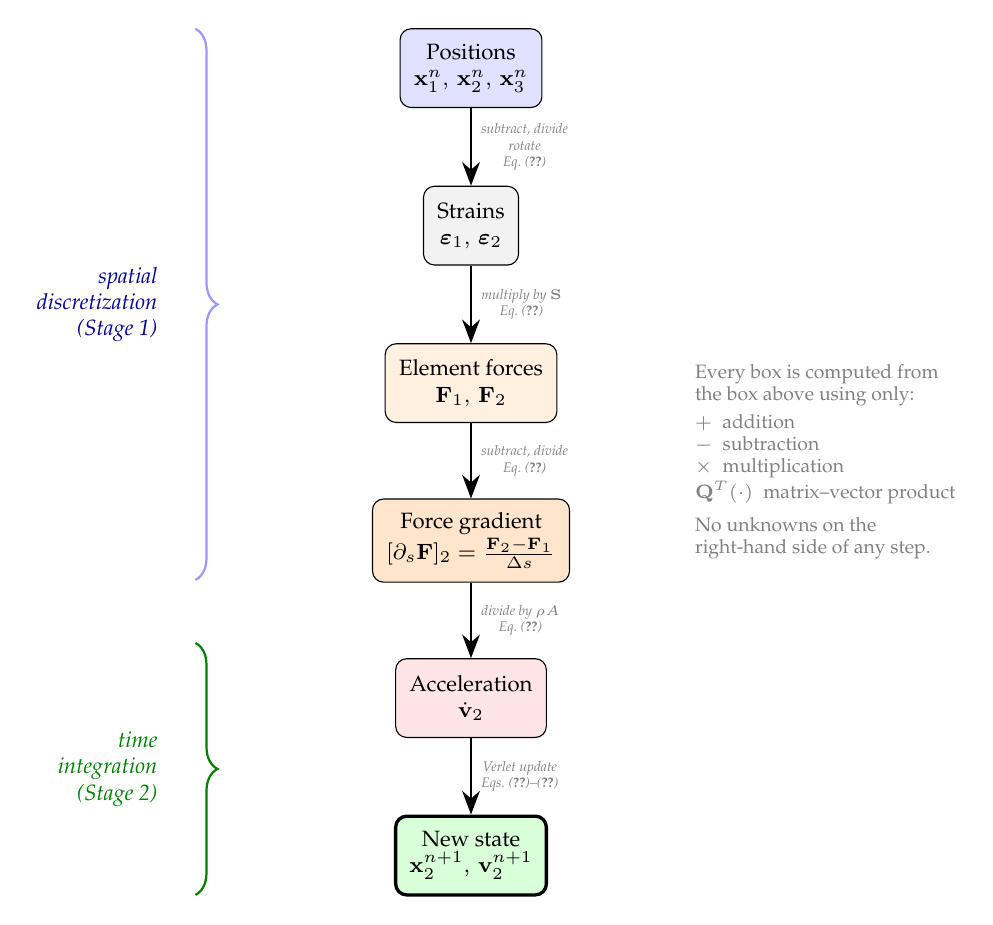
\begin{tikzpicture}[
  box/.style={rectangle, draw, rounded corners=4pt, minimum height=10mm, inner sep=5pt,
              font=\footnotesize, align=center},
  arr/.style={-{Stealth[length=3mm]}, thick},
  op/.style={font=\tiny\itshape, text=black!50, align=center},
  >=Stealth
]
  % Row 1: inputs
  \node[box, fill=blue!12] (pos) at (0, 0) {Positions\\$\vect{x}_1^n,\, \vect{x}_2^n,\, \vect{x}_3^n$};

  % Row 2: strains
  \node[box, fill=gray!10] (strain) at (0, -2.0)
    {Strains\\$\bm{\varepsilon}_1,\, \bm{\varepsilon}_2$};
  \draw[arr] (pos) -- node[right, op] {subtract, divide\\rotate\\Eq.~(\ref{eq:strain-example})} (strain);

  % Row 3: forces
  \node[box, fill=orange!12] (force) at (0, -4.0)
    {Element forces\\$\vect{F}_1,\, \vect{F}_2$};
  \draw[arr] (strain) -- node[right, op] {multiply by $\mat{S}$\\Eq.~(\ref{eq:constitutive-example})} (force);

  % Row 4: force gradient
  \node[box, fill=orange!20] (grad) at (0, -6.0)
    {Force gradient\\$[\partial_s \vect{F}]_2 = \frac{\vect{F}_2 - \vect{F}_1}{\Delta s}$};
  \draw[arr] (force) -- node[right, op] {subtract, divide\\Eq.~(\ref{eq:fd-force})} (grad);

  % Row 5: acceleration
  \node[box, fill=red!10] (accel) at (0, -8.0)
    {Acceleration\\$\dot{\vect{v}}_2$};
  \draw[arr] (grad) -- node[right, op] {divide by $\rho A$\\Eq.~(\ref{eq:accel-example})} (accel);

  % Row 6: new state
  \node[box, fill=green!15, line width=1.2pt] (newpos) at (0, -10.0)
    {New state\\$\vect{x}_2^{n+1},\, \vect{v}_2^{n+1}$};
  \draw[arr] (accel) -- node[right, op] {Verlet update\\Eqs.~(\ref{eq:verlet-x-example})--(\ref{eq:verlet-x2-example})} (newpos);

  % Side annotations
  \draw[decorate, decoration={brace, amplitude=8pt}, thick, blue!40]
    (-3.5, 0.5) -- (-3.5, -6.5)
    node[midway, left=10pt, font=\footnotesize\itshape, blue!60!black, align=right]
    {spatial\\discretization\\(Stage 1)};

  \draw[decorate, decoration={brace, amplitude=8pt}, thick, green!50!black]
    (-3.5, -7.3) -- (-3.5, -10.5)
    node[midway, left=10pt, font=\footnotesize\itshape, green!50!black, align=right]
    {time\\integration\\(Stage 2)};

  % Right annotation
  \node[font=\scriptsize, text=black!50, align=left] at (4.5, -5.0)
    {Every box is computed from\\the box above using only:\\[2pt]
     $+$\; addition\\
     $-$\; subtraction\\
     $\times$\; multiplication\\
     $\mat{Q}^T(\cdot)$\; matrix--vector product\\[4pt]
     No unknowns on the\\right-hand side of any step.};
\end{tikzpicture}
\end{center}

\noindent
Every arrow is addition, subtraction, multiplication, or a matrix--vector product.
At no point does an unknown quantity appear on the right-hand side of any expression.
This is what it means for a PDE to be ``solved'' by explicit evaluation: the continuous derivatives have been replaced by arithmetic on neighboring grid values, and the time derivative has been replaced by a forward step from the known state.

\subsection{The result: PDE becomes a system of ODEs}

After discretizing the domain and the spatial operators, all spatial dependence has been eliminated.
What remains is a system of ordinary differential equations in time:
\begin{equation}
  \dot{\vect{s}}(t) = \vect{g}\bigl(\vect{s}(t),\, \vect{a}(t)\bigr)
  \label{eq:mol-ode}
\end{equation}
where $\vect{g}: \Real^d \to \Real^d$ is a \emph{known, closed-form function} that encodes the entire spatial physics:
\begin{equation}
  \vect{g}(\vect{s}) = \underbrace{\text{geometry}}_{\vect{x}_i \to \vect{t}_e, \ell_e}
  \;\to\; \underbrace{\text{strains}}_{\vect{t}_e \to \varepsilon_e, \kappa_e}
  \;\to\; \underbrace{\text{constitutive law}}_{\varepsilon_e \to \vect{F}_e, \kappa_e \to \vect{M}_e}
  \;\to\; \underbrace{\text{force balance}}_{\mat{D}^T \vect{F}_e + \vect{f}_{\text{ext}}}
  \;\to\; \underbrace{\text{accelerations}}_{\vect{F}_{\text{net}} / ({\rho A})}
  \label{eq:g-pipeline}
\end{equation}

Every step in this pipeline is an explicit algebraic formula --- multiplication, addition, cross products, matrix--vector products.
No step requires solving an equation.
This is why the method-of-lines approach converts the PDE into something that can be ``solved'' by sequential evaluation.

\subsection{Comparison: how the three discretization families handle this}

Different discretization families (Section~\ref{sec:approaches}) differ in how they replace the spatial derivatives, but the end result is always the same --- a finite system that a computer can evaluate:

\begin{table}[H]
\centering
\renewcommand{\arraystretch}{1.3}
\begin{tabular}{@{}p{2.5cm}p{4cm}p{5cm}@{}}
\toprule
\textbf{Family} & \textbf{How it discretizes space} & \textbf{What the PDE becomes} \\
\midrule
Finite differences &
  Replace $\partial/\partial s$ with ratios of neighbor values on a grid &
  System of ODEs (if time left continuous) or algebraic equations (if time also discretized) \\[4pt]
Finite elements &
  Approximate $\vect{u}(s) \approx \sum_j c_j \phi_j(s)$ with basis functions; enforce PDE via weighted integrals &
  $\mat{M}\,\dot{\vect{c}} = \vect{f}(\vect{c})$ (mass matrix times rate = force vector) \\[4pt]
Spectral methods &
  Expand $\vect{u}(s) = \sum_k \hat{u}_k\, e^{ik\pi s/L}$; operate in frequency space &
  $\dot{\hat{\vect{u}}} = \vect{f}(\hat{\vect{u}})$ (ODEs for spectral coefficients) \\
\bottomrule
\end{tabular}
\end{table}

\noindent
PyElastica uses the first approach (finite differences on a staggered grid) because Cosserat rods are one-dimensional in space, making finite differences natural and efficient.
For more complex geometries (2D/3D), finite elements are preferred because they can handle irregular meshes.

% ===================================================================
\section{Why Elastica's Method Is Called ``Explicit''}
\label{sec:explicit}
% ===================================================================

The terms ``explicit'' and ``implicit'' refer to how the time integrator computes the next state.

\subsection{Definitions}

Consider an ODE system $\dot{\vect{s}} = \vect{g}(\vect{s}, t)$ with current state $\vect{s}^n$ at time $t^n$.

\paragraph{Explicit method.}
The next state is computed directly from the current state:
\begin{equation}
  \vect{s}^{n+1} = \Phi(\vect{s}^n, t^n, \Delta t)
  \label{eq:explicit-def}
\end{equation}
where $\Phi$ is a known, closed-form function.
The unknown $\vect{s}^{n+1}$ appears \emph{only on the left-hand side}.
Given $\vect{s}^n$, you \emph{evaluate} $\Phi$ to obtain $\vect{s}^{n+1}$.
No equation is solved.

\paragraph{Implicit method.}
The next state satisfies an equation that involves itself:
\begin{equation}
  \vect{s}^{n+1} = \Psi(\vect{s}^{n+1}, \vect{s}^n, t^n, \Delta t)
  \label{eq:implicit-def}
\end{equation}
The unknown $\vect{s}^{n+1}$ appears \emph{on both sides}.
You cannot simply evaluate the right-hand side --- you must \emph{solve} for $\vect{s}^{n+1}$, typically via Newton iteration.

\subsection{Concrete examples}

\begin{table}[H]
\centering
\renewcommand{\arraystretch}{1.3}
\begin{tabular}{@{}lll@{}}
\toprule
\textbf{Method} & \textbf{Update rule} & \textbf{Type} \\
\midrule
Forward Euler &
  $\vect{s}^{n+1} = \vect{s}^n + \Delta t\,\vect{g}(\vect{s}^n)$ &
  Explicit \\
Backward Euler &
  $\vect{s}^{n+1} = \vect{s}^n + \Delta t\,\vect{g}(\vect{s}^{n+1})$ &
  Implicit \\
Position Verlet &
  Eqs.~(\ref{eq:verlet-half})--(\ref{eq:verlet-full}) &
  Explicit \\
\bottomrule
\end{tabular}
\end{table}

\subsection{Position Verlet is explicit}

The Position Verlet scheme used by PyElastica consists of three substeps:
\begin{subequations}
\label{eq:verlet}
\begin{align}
  \vect{q}^{n+\frac{1}{2}} &= \vect{q}^n
    + \tfrac{1}{2}\,\Delta t\;\dot{\vect{q}}^n
  \label{eq:verlet-half} \\[4pt]
  \dot{\vect{q}}^{n+1} &= \dot{\vect{q}}^n
    + \Delta t\;\ddot{\vect{q}}\!\left(\vect{q}^{n+\frac{1}{2}}\right)
  \label{eq:verlet-vel} \\[4pt]
  \vect{q}^{n+1} &= \vect{q}^{n+\frac{1}{2}}
    + \tfrac{1}{2}\,\Delta t\;\dot{\vect{q}}^{n+1}
  \label{eq:verlet-full}
\end{align}
\end{subequations}

Every quantity on the right-hand side of each equation is \emph{already known} when that equation is evaluated:
\begin{itemize}
  \item Eq.~(\ref{eq:verlet-half}): uses $\vect{q}^n$ and $\dot{\vect{q}}^n$ (the current state).
  \item Eq.~(\ref{eq:verlet-vel}): uses $\dot{\vect{q}}^n$ and $\ddot{\vect{q}}(\vect{q}^{n+1/2})$. The acceleration is computed from $\vect{q}^{n+1/2}$, which was just determined in the previous line.
  \item Eq.~(\ref{eq:verlet-full}): uses $\vect{q}^{n+1/2}$ and $\dot{\vect{q}}^{n+1}$, both already computed.
\end{itemize}

\noindent
At no point does an unknown appear on both sides of an equation.
The entire substep is a \textbf{sequential evaluation} --- a chain of assignments, not a system of equations to solve.

% ===================================================================
\section{How Elastica Solves a PDE Through Sequential Evaluation}
\label{sec:how}
% ===================================================================

The key insight is a two-stage reduction:

\begin{center}
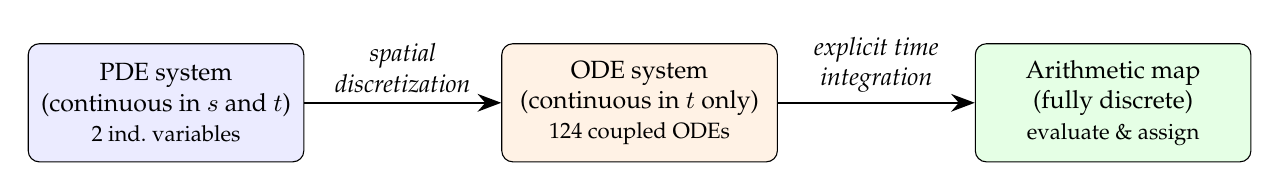
\begin{tikzpicture}[
  box/.style={draw, rounded corners=4pt, minimum height=1.5cm,
              minimum width=3.5cm, align=center, font=\small},
  arr/.style={-{Stealth[length=3mm]}, thick},
  lbl/.style={font=\small\itshape, align=center}
]
  \node[box, fill=blue!8] (pde) {PDE system \\ (continuous in $s$ and $t$) \\ {\footnotesize 2 ind.\ variables}};
  \node[box, fill=orange!10, right=2.5cm of pde] (ode)
    {ODE system \\ (continuous in $t$ only) \\ {\footnotesize 124 coupled ODEs}};
  \node[box, fill=green!10, right=2.5cm of ode] (map)
    {Arithmetic map \\ (fully discrete) \\ {\footnotesize evaluate \& assign}};

  \draw[arr] (pde) -- node[above, lbl] {spatial\\discretization} (ode);
  \draw[arr] (ode) -- node[above, lbl] {explicit time\\integration} (map);
\end{tikzpicture}
\end{center}

\subsection{Stage 1: Spatial discretization eliminates the spatial variable}

The Cosserat rod PDE contains two types of derivatives: $\partial/\partial s$ (spatial) and $\partial/\partial t$ (temporal).
Spatial discretization replaces all $\partial/\partial s$ derivatives with finite difference operators on the staggered grid ($N = 21$ nodes, $N_e = 20$ elements).

\paragraph{What the spatial derivatives become.}
Each continuous spatial derivative maps to a matrix--vector product:

\begin{table}[H]
\centering
\renewcommand{\arraystretch}{1.3}
\begin{tabular}{@{}lll@{}}
\toprule
\textbf{Continuous} & \textbf{Discrete} & \textbf{Operation} \\
\midrule
$\displaystyle\dds{\vect{F}}$ &
  $\mat{D}^T \vect{F}_e$ &
  Bidiagonal matrix $\times$ element force vector \\[6pt]
$\displaystyle\dds{\vect{M}}$ &
  $\mat{D}_v^T \bm{\tau}_v$ &
  Voronoi difference matrix $\times$ moment vector \\[6pt]
$\bm{\kappa}(s) - \bm{\kappa}_0(s)$ &
  $\kappa_e - \kappa_e^{\text{rest}}$ &
  Element-wise subtraction \\[4pt]
$\bm{\varepsilon}(s)$ &
  $\mat{Q}_e^T\,\Delta\vect{x}_e / \ell_e^{\text{rest}}$ &
  Rotation $\times$ finite difference \\
\bottomrule
\end{tabular}
\end{table}

\noindent
After this replacement, no spatial derivative remains.
The continuous PDE in $(s, t)$ has become a system of 124 coupled ODEs in $t$ alone:
\begin{equation}
  \dot{\vect{s}} = \vect{g}(\vect{s},\, \vect{a},\, t),
  \qquad \vect{s} \in \Real^{124}
  \label{eq:ode-system}
\end{equation}

The function $\vect{g}$ encodes all the spatial coupling: each node's acceleration depends on its neighbors through the difference operators $\mat{D}$ and $\mat{D}^T$.
But $\vect{g}$ is a \emph{closed-form function} --- given the current state $\vect{s}$, you can compute $\vect{g}(\vect{s})$ by evaluating a sequence of explicit formulas (geometry $\to$ strains $\to$ constitutive law $\to$ forces $\to$ accelerations).

\paragraph{Why this works.}
The difference matrices ($\mat{D}$, $\mat{D}^T$, $\mat{A}_v$, $\mat{D}_v$) are sparse, bidiagonal or tridiagonal.
A matrix--vector product $\mat{D}^T \vect{F}_e$ is just arithmetic: each entry is a weighted sum of two neighboring values.
The constitutive law $\vect{F} = \mat{S}(\bm{\varepsilon} - \bm{\varepsilon}_0)$ is an algebraic relation: multiply stiffness by strain.
None of these operations requires solving a system of equations.

\subsection{Stage 2: Explicit time integration eliminates the temporal variable}

With the ODE system (\ref{eq:ode-system}) in hand, an explicit integrator advances the state by one substep using only the \emph{current} (known) state:

\begin{equation}
  \vect{s}^{n+1} = \vect{s}^n + \Delta t \cdot \vect{h}(\vect{s}^n)
  \label{eq:explicit-step}
\end{equation}

where $\vect{h}$ involves evaluating $\vect{g}$ (for Verlet, at the half-step configuration).
Since $\vect{g}$ is a closed-form function and $\vect{s}^n$ is known, the entire right-hand side is computable by direct evaluation.

\paragraph{Contrast with implicit methods.}
An implicit integrator (e.g., backward Euler) writes:
\begin{equation}
  \vect{s}^{n+1} = \vect{s}^n + \Delta t \cdot \vect{g}(\vect{s}^{n+1})
  \label{eq:implicit-step}
\end{equation}
Now $\vect{s}^{n+1}$ appears on \emph{both sides}.
This is a system of 124 nonlinear equations in 124 unknowns, requiring Newton iteration to solve.
Each Newton step assembles the Jacobian $\partial\vect{g}/\partial\vect{s}$ and solves a linear system --- this is what makes implicit methods expensive per step.

\subsection{The complete picture: Elastica's substep as a function composition}

A single Verlet substep in Elastica is a composition of explicit operations:

\begin{equation}
  V_{\Delta t}: \quad
  \vect{s}^n
  \;\xrightarrow{\text{half-step}}\;
  \vect{q}^{n+1/2}
  \;\xrightarrow{\text{geometry}}\;
  (\vect{t}_e, \ell_e, \varepsilon_e)
  \;\xrightarrow{\text{constitutive}}\;
  (\vect{F}^{\text{int}}, \vect{M}^{\text{int}})
  \;\xrightarrow{\text{forces}}\;
  \ddot{\vect{q}}
  \;\xrightarrow{\text{update}}\;
  \vect{s}^{n+1}
  \label{eq:pipeline}
\end{equation}

Every arrow is a \emph{function evaluation}, not an equation to solve.
The entire pipeline is a deterministic map $\Real^{124} \to \Real^{124}$ computed in a single forward pass --- no iteration, no convergence check, no matrix inversion.

One RL control step composes $n_{\text{sub}} = 500$ of these maps:
\begin{equation}
  T(\vect{s}_t, \vect{a}_t) = \underbrace{V_{\Delta t} \circ \cdots \circ V_{\Delta t}}_{500}(\vect{s}_t;\, \vect{a}_t)
  \label{eq:transition-composition}
\end{equation}

% ===================================================================
\section{Why Explicit Methods Need Small Timesteps}
\label{sec:stability}
% ===================================================================

The price of avoiding an equation solve is a \textbf{stability constraint}.
Explicit methods are conditionally stable: if $\Delta t$ exceeds a critical value, the numerical solution grows unboundedly.

For the Cosserat rod, the critical timestep is set by the fastest wave (bending waves in the stiffest mode):
\begin{equation}
  \Delta t < C\,\sqrt{\frac{\rho A\,\Delta s^4}{EI}}
  \label{eq:cfl}
\end{equation}
where $\Delta s = L/N_e$ is the element length and $C$ is an order-unity constant.
With the project's default parameters, this gives $\Delta t_{\max} \approx 1.7 \times 10^{-3}$\,s, and Elastica uses $\Delta t = 10^{-3}$\,s (safely below the limit).

Implicit methods (backward Euler, Newmark) are \emph{unconditionally stable}: any $\Delta t$ produces a bounded solution.
This is why DisMech can use $\Delta t = 0.05$\,s (50$\times$ larger), but pays for it with a Newton solve at every step.

\begin{table}[H]
\centering
\caption{The explicit--implicit tradeoff.}
\label{tab:tradeoff}
\renewcommand{\arraystretch}{1.3}
\begin{tabular}{@{}lll@{}}
\toprule
& \textbf{Explicit (Elastica)} & \textbf{Implicit (DisMech)} \\
\midrule
Per-step cost & Low (evaluate formulas) & High (Jacobian + linear solve) \\
Step size & Small ($\Delta t = 0.001$\,s) & Large ($\Delta t = 0.05$\,s) \\
Steps per RL action & 500 & 1 \\
Stability & Conditional (CFL limit) & Unconditional \\
Solves an equation? & No & Yes (Newton iteration) \\
``Solver'' in the classical sense? & No & Yes \\
\bottomrule
\end{tabular}
\end{table}

% ===================================================================
\section{Implications for the Neural Surrogate}
\label{sec:surrogate}
% ===================================================================

The neural surrogate $f_\theta$ replaces the 500-step composition $T$ with a single forward pass.
Understanding \emph{what it replaces} clarifies the surrogate's role:

\begin{enumerate}
  \item \textbf{It does not replace a PDE solver.}
    Elastica was never solving the PDE in the traditional sense (no Newton iteration, no stiffness matrix).
    It was \emph{evaluating} 500 sequential maps.

  \item \textbf{It replaces a function composition.}
    The ground truth is $T = V_{\Delta t}^{500}$, a composition of 500 explicit maps.
    The surrogate $f_\theta$ approximates this composition in a single evaluation:
    \begin{equation}
      f_\theta(\vect{s}_t,\, \vect{a}_t) \approx T(\vect{s}_t,\, \vect{a}_t) - \vect{s}_t
      \label{eq:surrogate}
    \end{equation}

  \item \textbf{The ``difficulty'' is compositional, not algebraic.}
    Each individual Verlet substep is cheap and simple.
    What makes the transition operator expensive is that 500 substeps must be composed sequentially --- the output of each feeds into the next.
    The surrogate's value is collapsing this sequential composition into a single parallel computation (a neural network forward pass).
\end{enumerate}

% ===================================================================
\section{Summary}
\label{sec:summary}
% ===================================================================

\begin{enumerate}
  \item \textbf{``Explicit'' means the next state is computed by evaluation, not by solving an equation.}
    In Position Verlet, every right-hand side is already known when it is evaluated.
    The unknown $\vect{s}^{n+1}$ never appears on the right-hand side.

  \item \textbf{The standard PDE solver uses implicit time integration with Newton iteration.}
    This is what DisMech does and what most engineers mean by ``solving a PDE.''
    The Newton solve --- assembling the Jacobian and factorizing a sparse linear system --- is the computational bottleneck.

  \item \textbf{Elastica solves a PDE through the method of lines plus explicit integration.}
    Spatial discretization converts $\partial/\partial s$ into matrix--vector products (Stage~1).
    Explicit time integration converts $\partial/\partial t$ into sequential evaluation (Stage~2).
    After both stages, the entire PDE simulation is reduced to a chain of arithmetic operations --- no equation is ever solved.
    The price is a CFL stability constraint that forces small timesteps.
\end{enumerate}

\noindent
The neural surrogate replaces this chain of 500 arithmetic maps with a single forward pass, trading the CFL-enforced sequential composition for a learned parallel computation.

% ===================================================================
% References
% ===================================================================
\begin{thebibliography}{9}

\bibitem{strikwerda2004finite}
J.~C. Strikwerda,
\textit{Finite Difference Schemes and Partial Differential Equations},
2nd ed., SIAM, 2004.

\bibitem{leveque2007finite}
R.~J. LeVeque,
\textit{Finite Difference Methods for Ordinary and Partial Differential Equations},
SIAM, 2007.

\bibitem{hairer2006geometric}
E.~Hairer, C.~Lubich, and G.~Wanner,
\textit{Geometric Numerical Integration: Structure-Preserving Algorithms for Ordinary Differential Equations},
2nd ed., Springer, 2006.

\bibitem{gazzola2018forward}
M.~Gazzola, L.~H. Dudte, A.~G. McCormick, and L.~Mahadevan,
``Forward and inverse problems in the mechanics of soft filaments,''
\textit{Royal Society Open Science}, vol.~5, no.~6, 2018.

\bibitem{bergou2008discrete}
M.~Bergou, M.~Wardetzky, S.~Robinson, B.~Audoly, and E.~Grinspun,
``Discrete elastic rods,''
\textit{ACM Transactions on Graphics (SIGGRAPH)}, vol.~27, no.~3, 2008.

\end{thebibliography}

\end{document}
